%!TEX root = ../../thesis.tex

\ac{QCD} is the theory of the strong interaction, describing coloured particles (quarks 
and gluons) \cite{Ellis:1996}. Two crucial features of \ac{QCD} are \textit{confinement} 
and \textit{asymptotic freedom}. Confinement refers to the observation that quarks and 
gluons are only found within hadrons, and never as isolated states. Asymptotic freedom 
states that, within the hadron, the constituent partons are relatively free to move. Both 
concepts can be understood in terms of a running coupling constant.



\subsection{Renormalisation and the running coupling}
\label{sec:qcd:renormalisation}

When calculating observables within perturbative quantum field theory, ultraviolet (UV) 
divergences are often introduced by Feynman diagrams containing loops. Through careful 
consideration, these UV divergences can be absorbed into renormalised definitions of the 
coupling constant and particle masses. The idea is that the `bare' quantities contain 
compensating divergences, such that the physically measurable quantities are finite:
\begin{equation}
	g_{\text{physical}} = g_{\text{bare}} + \delta g
	\quad\quad\text{and}\quad\quad
	m_{\text{physical}} = m_{\text{bare}} + \delta m
\end{equation}
where $\delta g$ and $\delta m$ are the loop contributions. This procedure is known as 
\textit{renormalisation}.

It is necessary to introduce an unphysical \textit{renormalisation scale} $\mu_R$, above 
which loops are absorbed into renormalised quantities, and below which loops are 
calculated in perturbation theory. Clearly couplings and masses will depend upon $\mu_R$,
though physical observables must not -- however, truncation of the perturbative series 
results in a residual $\mu_R$ dependence. Usually $\mu_R$ is chosen to be the energy 
scale $Q$ of the process under consideration, leading to the concept of a `running 
coupling constant'.

For \ac{QCD}, the coupling constant \alphaS is shown in \Figure~\ref{fig:alpha_s}. At 
small scales (large distances), \alphaS is large and the theory is non-perturbative. 
Though not analytically proven\footnote{
	A mathematically rigorous proof of confinement is one of seven Millennium Prize 
	Problems of the Clay Mathematics Institute, with a bounty of \$1,000,000.
}, confinement has been verified by lattice \ac{QCD} in this regime \cite{Wilson:1974}. 
At high scales (small distances), \alphaS is small -- this is asymptotic freedom 
\cite{Gross:1973,Politzer:1973}. Note that \alphaEM in \acs{QED} exhibits an opposing 
trend, though remains perturbative at accessible energies.
\begin{figure}
	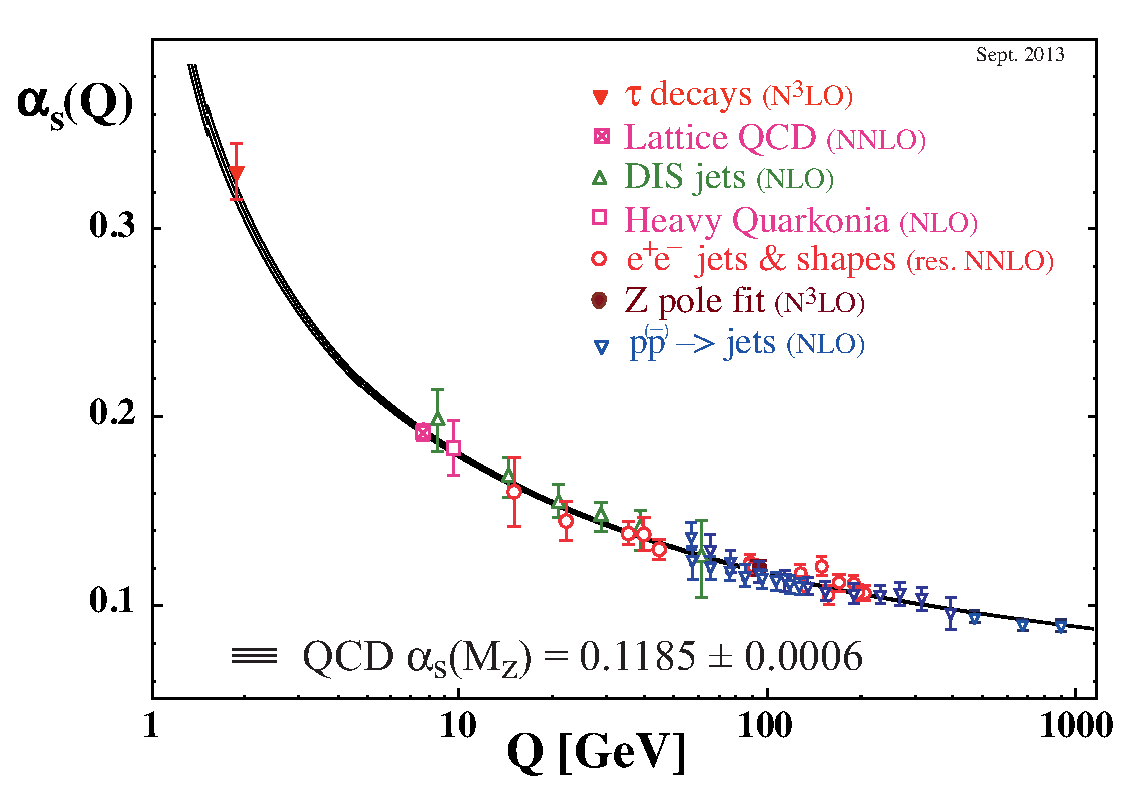
\includegraphics[width=\mediumfigwidth]{tex/tools/alpha_s}
	\caption{The running of the strong coupling constant \alphaS with energy scale $Q$ 
	\cite{PDG:2012}. Experimental measurements at various scales are also shown.}
	\label{fig:alpha_s}
\end{figure}



\subsection{Perturbative QCD}
\label{sec:qcd:pqcd}

Most \acs{LHC} processes of interest involve large momentum transfer where partons are 
asymptotically free. Thus, parton-level cross sections may be calculated with Feynman 
diagrams as a convergent perturbative series in \alphaS
\begin{equation}
	\hat{\sigma} = \sum\limits_{m=0}^{\infty} \alpha_S^{k+m} \hat{\sigma}^{(m)}
\end{equation}
where the hat denotes a parton-level quantity, $k$ is the number of \ac{QCD} vertices at 
tree-level, and $\hat{\sigma}^{(m)}$ is the $m$th order contribution to the cross section.

As mentioned above, the cross section $\hat{\sigma}$ is independent of the 
renormalisation scale
\begin{equation}
	\frac{\d{\hat{\sigma}}}{\d{\mu_R}} = 0 \,.
	\label{eq:xs_rge}
\end{equation}
However, real-life calculations always truncate the series after $n$ terms, leaving a 
residual $\mu_R$ dependence. Inserting the truncated series into (\ref{eq:xs_rge}), we 
find that
\begin{equation}
	\frac{\d{}}{\d{\mu_R}} \sum\limits_{m=0}^{n} \alpha_S^{k+m} \hat{\sigma}^{(m)}
	= \ofOrder{\alpha_S^{k+n+1}}
\end{equation}
and it follows that the residual $\mu_R$ dependence can be used to probe the effect of 
missing higher order terms in the series.

In addition to the UV divergences handled by renormalisation, infrared (IR) divergences 
arise from the soft and collinear emission of massless gluons. However, the 
Kinoshita-Lee-Nauenberg theorem states that these will cancel with IR divergences in 
corresponding loop diagrams \cite{Kinoshita:1962,Lee:1964}.



\subsection{Parton shower}
\label{sec:qcd:ps}

\subsection{Parton distribution functions}
\label{sec:qcd:pdf}

dependence on muF is DGLAP equation

\begin{equation}
	\sigma_{\HepProcess{\Pproton \Pproton \HepTo X}}\parenths{P_1, P_2} = 
	\sum\limits_{a, b} \! \int \! \d{x_1} \d{x_2} \,
	f_a \parenths{x_1, \mu_F^2} f_b \parenths{x_2, \mu_F^2} \,
	\hat{\sigma}_{\HepProcess{ab \HepTo X}} \parenths{p_1, p_2, \alphaS\parenths{\mu_R^2}, \frac{Q^2}{\mu_F^2}, \frac{Q^2}{\mu_R^2}} 
\end{equation}
